\documentclass[a4paper,12pt]{article}

%%% Работа с русским языком
\usepackage{cmap}					% поиск в PDF
\usepackage{mathtext} 				% русские буквы в формулах
\usepackage[T2A]{fontenc}			% кодировка
\usepackage[utf8]{inputenc}			% кодировка исходного текста
\usepackage[english,russian]{babel}	% локализация и переносы
\usepackage{xcolor}
\usepackage{hyperref}
 % Цвета для гиперссылок
\definecolor{linkcolor}{HTML}{799B03} % цвет ссылок
\definecolor{urlcolor}{HTML}{799B03} % цвет гиперссылок

\hypersetup{pdfstartview=FitH,  linkcolor=linkcolor,urlcolor=urlcolor, colorlinks=true}

%%% Дополнительная работа с математикой
\usepackage{amsfonts,amssymb,amsthm,mathtools} % AMS
\usepackage{amsmath}
\usepackage{icomma} % "Умная" запятая: $0,2$ --- число, $0, 2$ --- перечисление

%% Номера формул
%\mathtoolsset{showonlyrefs=true} % Показывать номера только у тех формул, на которые есть \eqref{} в тексте.

%% Шрифты
\usepackage{euscript}	 % Шрифт Евклид
\usepackage{mathrsfs} % Красивый матшрифт

%% Свои команды
\DeclareMathOperator{\sgn}{\mathop{sgn}}

%% Перенос знаков в формулах (по Львовскому)
\newcommand*{\hm}[1]{#1\nobreak\discretionary{}
{\hbox{$\mathsurround=0pt #1$}}{}}
% графика
\usepackage{graphicx}
\graphicspath{{pictures/}}
\DeclareGraphicsExtensions{.pdf,.png,.jpg}
\author{Бурмашев Григорий, БПМИ-208}
\title{}
\date{\today}
\begin{document}
{\Large \begin{center}
Бурмашев Григорий. 208. Матан -- 13(?)
\end{center}}

\begin{center}
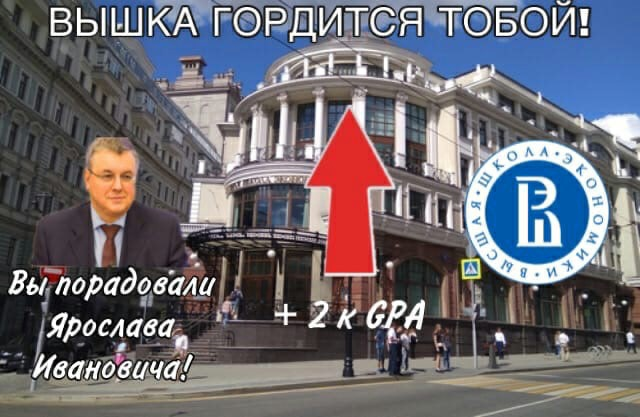
\includegraphics[scale=0.6]{1.jpg}
\end{center}
\clearpage
\section*{Номер 9}
\subsection*{a)}
\[
f(x, y) = x^2 \ln \left(x^2 + y^2 \right)
\]
Расписываем через полярные координаты:
\[
r^2 \cdot \cos^2 \phi  \cdot \ln(r^2 \cos^2 \phi + r^2 \sin^2 \phi) = r^2 \cos^2 \phi \cdot \ln (r^2) =  r^2 \cos^2 \phi \cdot 2\ln (r) 
\]
Теперь смотрим на предел ($\cos^2$ ограничен очев):

\[
\lim_{r \rightarrow 0} r^2 \cos^2 \phi \cdot2 \ln r = 2 \lim_{r \rightarrow 0} \left( r^2 \cos^2 \phi \cdot \ln r  \right) =  2 \lim_{r \rightarrow 0} \left(\cos^2 \phi \cdot  \frac{ \ln r}{\frac{1}{r^2}} \right)
\]
Получили штуку как на семинаре, ограниченный косинус умножаем на что-то, если это что-то стремится к нулю, тогда все круто (весь предел равен нулю), посмотрим:
\[
\lim_{r \rightarrow 0} \left( \frac{ \ln r}{\frac{1}{r^2}} \right) = \left[\frac{\infty}{\infty}\right] = \lim_{r \rightarrow 0} \left( \frac{ \frac{1}{r} }{-\frac{2}{r^3}} \right) = \lim_{r \rightarrow 0} -\frac{r^2}{2} = 0
\]
А значит:
\[
2 \lim_{r \rightarrow 0} \left(\cos^2 \phi \cdot  \frac{ \ln r}{\frac{1}{r^2}} \right) = 0
\]
\[
\lim_{\begin{matrix} x \rightarrow 0 \\ y \rightarrow 0 \end{matrix}} \left(x^2 \ln (x^2 + y^2) \right) = 0
\]
Чтобы была непрерывность значение функции в точке должно совпадать с пределом, т.к $\ln(0)$ неопр, то мы можем доопределить до непрерывной функции $f$ следующим образом:
\[
f = \begin{cases}
x^2 \ln (x^2 + y^2) , \text{ кроме (0, 0)} \\
0, \; \text{ в } (0, 0)
\end{cases}
\]
\\
{\Large \begin{center}
\textbf{Ответ: } возможно
\[
f = \begin{cases}
x^2 \ln (x^2 + y^2) , \text{ кроме (0, 0)} \\
0, \; \text{ в } (0, 0)
\end{cases}
\]
\end{center}}

\clearpage
 \subsection*{b)}
\[
f(x, y) = \frac{x^2 + y}{\sqrt{x^2 + y^2}}
\]
Расписываем через полярные координаты:
\[
f(x, y) = \frac{r^2 \cos ^2 \phi + r \sin \phi}{\sqrt{r^2\cos^2\phi + r^2 \sin^2 \phi}} = \frac{r(r \cos^2\phi  + \sin \phi)}{r} = r\cos^2 \phi + \sin \phi
\]
Получили штуку почти как на семе,  $r\cos^2 \phi$ к нулю, у $ \sin \phi$ предела вообще нет, значит доопределить до непрерывной функции мы не сможем
{\Large \begin{center}
\textbf{Ответ: } невозможно
\end{center}}
\section*{Номер 10}
\subsection*{a)}
\[
f(x, y) = \sqrt[3]{4x^2 + y^2}
\]
Пускай $h_1 = -0.2, h_2 = 0.3$. Тогда расписываем аналогично семинару:
\[
\triangle f = f(1 + h_1, 2 + h_2) - f(1, 2) = \sqrt[3]{4(1+h_1)^2 + (2+h_2)^2} - \sqrt[3]{4 + 4} =
\]
\[
=
 \sqrt[3]{4 h_1^2 + 8 h_1 + h_2^2 + 4 h_2 + 8} - 2 = \sqrt[3]{8\left(\frac{h_1^2}{2} + h_1 + \frac{h_2^2}{8} + \frac{h_2}{2} + 1 \right)}
\]
\[
=
2\left(1 + h_1 + \frac{h_2}{2} + \frac{h_1^2}{2} + \frac{h_2^2}{8} \right)^{\frac{1}{3}} - 2 = 2 \left(1 + \frac{1}{3}\left(h_1 + \frac{h_2}{2} \right) +  \overline{o}(\sqrt[3]{\frac{h_1^2}{2} + \frac{h_2^2}{8}})  \right) - 2 = 
\]
\[
= \frac{2}{3}h_1 + \frac{1}{3}h_2 +  \overline{o}\left(\sqrt[3]{h_1^2+ h_2^2}\right)
\]
Тогда получаем:
\[
df = \frac{2}{3} \cdot (-0.2) + \frac{1}{3} \cdot (0.3) = -\frac{1}{30}
\]
{\Large \begin{center}
\textbf{Ответ: } $- \frac{1}{30}$
\end{center}}
\clearpage
\subsection*{b)}
\[
f(x, y) = x^3 y - xy^3
\]
\[
\triangle f = f(1 + h_1, 2 + h_2) - f(1, 2) = (1+h_1)^3(2+h_2) - (1+h_1)(2+h_2)^3 + 6
\]
Раскрываем все скобки:
\[
(1+h_1)^3(2+h_2) - (1+h_1)(2+h_2)^3 + 6 = h_2 h_1^3 + 2 h_1^3 + 3 h_2 h_1^2 + 6 h_1^2 -
\]
\[
-
 h_2^3 h_1 - 6 h_2^2 h_1 - 9 h_2 h_1 - 2 h_1 - h_2^3 - 6 h_2^2 - 11 h_2 - 6 + 6
\]
Все ненужные множители закидываем под $ \overline{o}\left(\sqrt{h_1^2+ h_2^2}\right)$, оставляем только коэффы при $h_1$ и $h_2$:
\[
-2h_1 - 11h_2 + \overline{o}\left(\sqrt{h_1^2+ h_2^2}\right)
\]
Тогда получаем:
\[
df = -2 \cdot (-0.5) - 11 \cdot (0.8) = -7.8
\]
{\Large \begin{center}
\textbf{Ответ: } -7.8 
\end{center}}
\clearpage
\section*{Номер 11}
\subsection*{a)}
\[
f(x, y) = x^2 + y^2
\]
\[
\frac{\sigma f}{\sigma x} =  2x + 0
\]
\[
\frac{\sigma y}{\sigma x} = 2y + 0
\]
Тогда:
\[
df = (2x) \,dx + (2y) \,dy 
\]
{\Large \begin{center}
\textbf{Ответ: } 
\[
df = (2x) \,dx + (2y) \,dy 
\]
\end{center}}
\subsection*{b)}
\[
f(x, y) = x^y + y^x
\]
\[
\frac{\sigma f}{\sigma x} = y \cdot x^{y -1 } + \ln(y) \cdot y^x
\]
\[
\frac{\sigma f}{\sigma y} = \ln (x) \cdot x^y + x \cdot y^{x-1}
\]
Тогда :
\[
df = \left(y \cdot x^{y -1 } + \ln(y)\cdot y^x\right) \, dx + \left(\ln (x) \cdot x^y + x \cdot y^{x-1}\right) \, dy\
\]
{\Large \begin{center}
\textbf{Ответ: } 
\[
df = \left(y \cdot x^{y -1 } + \ln(y)\cdot y^x\right) \, dx + \left(\ln (x) \cdot x^y + x \cdot y^{x-1}\right) \, dy\
\]
\end{center}}
\end{document}
